%----------------------------------------------------------------------------------------
%	PACKAGES AND OTHER DOCUMENT CONFIGURATIONS
%----------------------------------------------------------------------------------------

\documentclass[a4paper, 12pt]{article} % Font size (can be 10pt, 11pt or 12pt) and paper size (remove a4paper for US letter paper)

\usepackage[protrusion=true,expansion=true]{microtype} % Better typography
\usepackage{graphicx} % Required for including pictures
\usepackage{wrapfig} % Allows in-line images
\usepackage{multirow}

%\usepackage{mathpazo} % Use the Palatino font
\usepackage[T1]{fontenc} % Required for accented characters
\linespread{1.04} % Change line spacing here, Palatino benefits from a slight increase by default


% Included by Jack
\usepackage[
%width=16cm, 
left=1.5cm,
right=1.5cm,
top=2.5cm, 
bottom=2.5cm
]{geometry}
\usepackage{hyperref}
\usepackage{float}
\usepackage{fancyhdr}
\usepackage{cleveref}
\usepackage{subfig}
\usepackage[super]{nth}
\usepackage{setspace}

% for drawing lines
\usepackage{tikz}

% for gantt chart
\usepackage{pgfgantt}
\usepackage{xcolor}
\usepackage{color}
\definecolor{lblu}{RGB}{0,112,210}
\definecolor{blu}{RGB}{0,56,158}
\definecolor{gren}{RGB}{132,235,176}
\definecolor{purp}{RGB}{213,174,212}
\definecolor{yell}{RGB}{255,255,0}

\usepackage[
backend=bibtex,
style=numeric,
citestyle=numeric,
sorting=none,
maxnames=2
]{biblatex}
\addbibresource{mendeley.bib}
% Some field suppression via options
\ExecuteBibliographyOptions{isbn=false,url=false,doi=false,eprint=false}

\graphicspath{{images/}}

% Header and footer commands
\pagestyle{fancy}
\fancyhf{}
\rhead{Jack Leland}
\lhead{\textsc{Third Year Progress Report}}
\cfoot{\thepage}

\makeatletter
\renewcommand{\@listI}{\itemsep=0pt} % Reduce the space between items in the itemize and enumerate environments and the bibliography
\renewcommand*{\bibfont}{\tiny}


\renewcommand{\maketitle}{ % Customize the title - do not edit title and author name here, see the TITLE block below
\begin{minipage}{0.3\linewidth}
	\begin{flushleft}
%		\vspace{-95pt}
		\vspace{-12ex}
		\hspace{-17pt}
\includegraphics[width=1\linewidth]{Logos/Liverpool.jpg} \\
		\vspace{10pt}
		\hspace{-20pt}
\includegraphics[width=1\linewidth]{Logos/cdt_logo_text_black.png} \\
		
		
%		\vspace{10pt}
%		\hspace{-20pt}\includegraphics[width=1\linewidth]{CCFE.jpg} 		
		\vfill
	\end{flushleft}
\end{minipage}
\hfill
\begin{minipage}{0.65\linewidth}
	\begin{flushright} % Right align
		\vspace{-5ex}
		{\LARGE\@title} % Increase the font size of the title
		
		\vspace{10pt} % Some vertical space between the title and author name
		
		{\large\@author} % Author name
		
		\vspace{20pt}
		\@date % Date
		
%		\vspace{40pt} % Some vertical space between the author block and abstract
	\end{flushright}
\end{minipage}
\vspace{15pt} % Some vertical space between the abstract and first section
}
\newcommand{\spacer}{\rule{0pt}{3ex}}

%----------------------------------------------------------------------------------------
%	TITLE
%----------------------------------------------------------------------------------------

\title{\textbf{Third Year Progress Report} \\
		Measurements and particle-in-cell simulations of MAST-U flush-mounted Langmuir probes} % Subtitle

\author{\textsc{Jack Leland} % Author
	\\ {\textit{University of Liverpool, Brownlow Hill, Liverpool, L69 3GJ}}
	\\ \href{mailto:j.leland@liverpool.ac.uk}{j.leland@liverpool.ac.uk}
	} % Institution

\date{\today} % Date

%----------------------------------------------------------------------------------------

\begin{document}

\maketitle % Print the title section
\thispagestyle{plain}

%----------------------------------------------------------------------------------------
%	ABSTRACT AND KEYWORDS
%----------------------------------------------------------------------------------------

%\renewcommand{\abstractname}{Summary} % Uncomment to change the name of the abstract to something else

\begin{abstract}
Novel divertor configurations are being explored as a possible solution to the heat exhaust problem in tokamaks.
Detailed knowledge of temperature and density in these divertors is therefore essential when testing the effectiveness of the heat mitigation provided by the configurations.
850 Langmuir probes have been installed in the plasma facing components (PFCs) of MAST-U however their analysis will be complex owing to the challenges associated with the sensitivity of flush mounted probes to field line incidence angles. 
Detailed 2 and 3 dimensional particle-in-cell simulations are being carried out, using the particle-in-cell code SPICE, of a variety of different Langmuir probe tip geometries.
By simulating the voltage sweep of a probe in a prescribed plasma environment, the measured current-voltage characteristic can be compared to the specified temperature and density. 
Two experimental trips to Magnum-PSI in the Netherlands were also carried out to verify that the angled tip design, used on the probes in MAST-U, works at the grazing angles of incidence expected in the MAST-U divertor. 
The data from these experiments and the simulations will be compared and used to make modifications to the current Langmuir probe theory to properly account for field line angle effects and 3D tip geometries.
The updated model can then be applied to the interpretation of flush mounted Langmuir probe data from MAST-U.
 
\end{abstract}

%\hspace*{3,6mm}\textit{Keyswords:} lorem , ipsum , dolor , sit amet , lectus % Keywords

%\vspace{15pt} % Some vertical space between the abstract and first section

%\tableofcontents
%------------------------------------------------------------------------------------
%	ESSAY BODY
%------------------------------------------------------------------------------------


\section{\label{sec:intro}Introduction}

\subsection{\label{subsec:tokamaks}Tokamaks}
	Fusion is a potential candidate for base-load commercial energy production due to its lack of greenhouse gas emissions, high power output, abundant fuel and lack of long-lived radioactive waste.
%	A Deuterium-Tritium (DT) fuel mixture must be heated to high enough temperatures to create collisions of sufficient energy to allow fusion to take place. 
%	The equation for this reaction is:
%	\begin{equation}
%	\label{eq:DTEq}
%	{}^{2}_{1}D + {}^{3}_{1}T \rightarrow   {}^{4}_{2}He (3.5 MeV) + {}^{1}_{0}n (14.1 MeV)
%	\end{equation} 
%	The temperatures required ($\sim$ 200 eV for DT) will ionise the fuel mixture into a plasma, meaning that the individual charged components can be manipulated and confined by magnetic fields.
	One of the methods proposed for confining the fusion reaction is the use of magnetic fields, known as magnetic confinement fusion (MCF).
	This can be done using several techniques, the most widely used of which is the Tokamak; a toroidal magnetic device comprised of a combination of toroidal and poloidal magnetic fields in a helical shape. 
	This setup is being developed with the aim of confining the plasma for a long enough time to allow net energy to be extracted from the fusion reaction and delivered to the grid.  
	
\subsection{\label{subsec:exhaust}The Exhaust Problem and MAST-Upgrade}
	A necessary consequence of the magnetic containment of a plasma within a vessel, such as a tokamak, is the existence of open field lines, i.e. field lines which impinge on surfaces. 
	Particles orbiting along open field lines will therefore impact on these surfaces, meaning these field lines create an avenue for heat \& particles to flow out of the plasma and be deposited onto surfaces.
	This can be helpful as it allows the removal of impurities - notably helium `ash', a by product of the Deuterium-tritium (DT) fusion reaction - however it is usually necessary to physically separate the impinged surfaces from the core plasma to reduce the opposing flow of sputtered impurities into the core which radiate away heat. 
	This can be done with either a limiter or a divertor\cite{Wesson2011}, with modern devices almost exclusively using divertors because of (a) the reduced sputtering of impurities into the core, and (b) access to H-mode - a mode of operation with higher confinement of particles in the core \cite{Itoh1989}.
	
%	  usually done with use of a divertor (\cref{fig:divertor}), where the targets are separated from the core plasma by a magnetic null point, or X-point.
%	The points at which the separatrix - the line separating the closed and open field lines - hit the target plates are called strike points.
%	These strike points will experience the highest heat and particle fluxes from the core plasma as particles cross the separatrix and flow towards the target through the scrape-off layer.
%	
%	Divertors have been used for decades with great success, allowing for more stable plasmas to be created. 
	However, when scaling Tokamaks to the size required for commercial electricity generation, the divertor target plates will experience very high heat fluxes because of the high core temperature required.  
	Dealing with and mitigating these heat fluxes is one of the key challenges currently standing in the way of commercial fusion power for toroidal devices\cite{Romanelli2012}. 	 
	
%\subsection{\label{subsec:mast}MAST-Upgrade}
	\begin{wrapfigure}[17]{rt}{6cm}
		\centering
		\vspace{-10pt}
		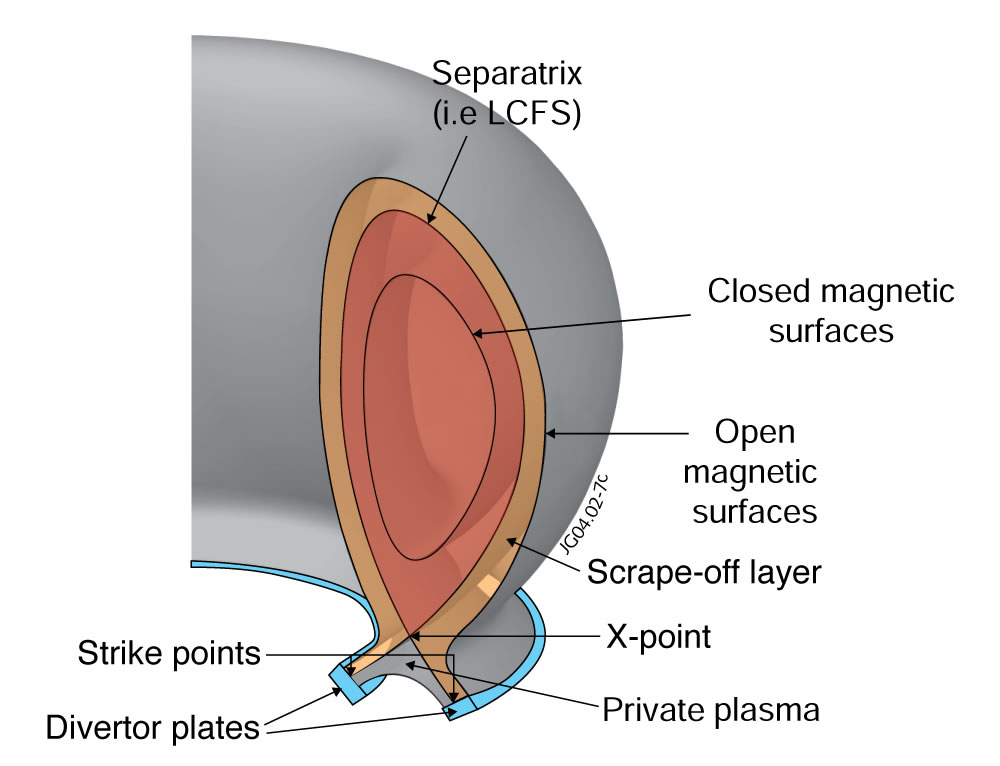
\includegraphics[width=1.0\linewidth]{IllustrativeFigures/divertor.jpg}
		\caption{\label{fig:divertor}A diagram of the regions within a tokamak plasma, including the separatrix and the divertor, separated from the core plasma by the X-point.}
	\end{wrapfigure}
	A proposed mitigation technique for the heat exhaust problem is the use of divertor configurations which allow for reduced heat flux to plasma facing components (PFCs). 
	MAST-Upgrade (MAST-U) at CCFE has been designed as an experiment to test several aspects of divertor physics, namely the use of a closed divertor with Super-X capability \cite{Valanju2009}.
	The closed aspect of the divertor means that it is separated from the main chamber by a baffle, and therefore more effective at restricting the flow of impurities and neutrals into the core, improving confinement. 
	The higher neutral pressure in the closed divertor also enhances the amount of energy loss via radiation, dissipating the power hitting the target plates.
	The Super-X configuration reduces heat flux further by extending the plasma out radially, increasing both the size of the strike point, so the same power is spread over a wider area; and the flight time of particles in the divertor, allowing them to lose energy over a longer period of time.
%	Lower neutral pressure in the core results in higher confinement and easier access to H-mode.
%	A detached plasma should also be easier to access, which involves having an increased neutral density in the divertor which increases radiation of energy from the plasma before it hits the target.
%	\begin{wrapfigure}[16]{rt}{7cm}
%		\centering
%		\vspace{-1.65cm}
%		\subfloat[]{\includegraphics[width=0.4\linewidth]{IllustrativeFigures/MastDivertorZoom.png}}
%		\hspace{10pt}
%		\subfloat[]{\includegraphics[width=0.4\linewidth]{IllustrativeFigures/LPLocations.png}}
%		\caption{Diagrams of (a) the magnetic flux of the Super-X configuration in MAST-U and (b) the locations of the Langmuir probe arrays in the MAST-U divertor (right).}
%		\label{fig:mast_divertor}
%	\end{wrapfigure} 

%	The combination of the closed divertor and the Super-X should allow for more effective control of the heat flux to the divertor tiles.
%	It is therefore necessary to understand, with great detail, what goes on in the MAST-U divertor when it is tested experimentally to ensure that the models predicting the behaviour of the plasma are valid. 
%	We therefore require detailed measurements of the density and temperature of the plasma in this region, which must be gained through diagnostic techniques.

\subsection{\label{subsec:lps}Langmuir Probes and Flush Mounting}
	Langmuir probes are a widely used diagnostic in plasma physics to measure electron temperature ($T_e$) and density ($n_e$). 
	In tokamaks they are limited to measuring plasma parameters near to the PFCs and the edge due to the extreme nature of the plasmas involved. 
	They are thus regularly flush mounted to reduce the incident heat flux to the probe tips and reduce erosion. 
	Flush mounted probes (FMPs) are however notoriously difficult to interpret in strongly magnetised plasmas \cite{Matthews1994}, notably because of the strong dependence on incidence angle of the magnetic field on the resultant shape of the current-voltage (IV) characteristic.
	
	At grazing angles of incidence, routinely found in tokamaks, sheath expansion becomes a dominant factor in the determination of the effective collection area ($A_{eff}$) of the probe \cite{Bergmann1994}. 
	Small uncertainties in the angle can therefore have large effects on the amount of sheath expansion experienced by the probe and therefore the shape of the IV characteristic.
	On top of this, magnetised probe theory is only valid when the projected probe extent is greater than the local Debye length and Larmor radius \cite{Gunn1995}. 
	The form of the IV characteristic, taking these effects into account, was developed by Bergmann \cite{Bergmann2002} and is as follows:
	\begin{equation}
	\label{eq:ivcurvesheathexp}
	\frac{I}{I_{i,sat}} =  1 + a |V|^{\frac{3}{4}} - \exp\left({-V}\right) \qquad \textnormal{with} \qquad  V = \bigg(\frac{e(V_p - V_f)}{k_B T_e}\bigg)
	\end{equation}
	where $I$ is the measured current, $I_{i,sat}$ is the ion saturation current, $V_p$ and $V_f$ are the probe and floating potentials respectively, $e$ is the charge on an electron and $k_B$ is the Boltzmann constant. 
	Bergmann's, and later Murphy-Sugrue's \cite{Murphy-Sugrue2017}, contribution to this equation is the addition of a sheath expansion term, $a$, which takes into account the incidence angle of the magnetic field $\theta$. 
	It is of the form
	\begin{equation}
	\label{eq:sheathexpparam}
	a =  \frac{c_1 + c_2  \cot{(\theta)}}{\sin^{\frac{1}{2}}{(\theta})} \frac{\lambda_D}{L + g}
	\end{equation}
	where $c_1$ and $c_2$ are coefficients of the lateral and frontal expansion of the sheath respectively, $\lambda_D$ is the Debye length of the plasma, $L$ is the length of the probe and $g$ is the size of the gaps either side of the probe.
	
	These issues have been previously mitigated on JET\cite{Monk1996} and DIII-D by angling the probe tip with respect to the incident magnetic field to increase the projected probe area and therefore lower the dependence on small changes of angle. 
	A similar probe tip has been designed for use in the divertor of the MAST-U tokamak at CCFE \cite{Harrison}, with 850 probes of this type installed throughout the PFCs.
	
\subsection{\label{subsec:motivation}PhD Project}
	As the collection area of the probe is essential to the calculation of the current density of the flux tube, getting measurements of $n_e$ becomes highly dependent on knowing the incidence angle and using this to calculate the area of the probe.
	This is also true for $T_e$, but to a lesser extent, as this is more dependent on orbits than small changes in collection area. 
	The main aim of this PhD project is to simulate the FMPs that will be used in the PFCs of MAST-U, using a 2D/3D3V particle-in-cell (PIC) simulation code called SPICE \cite{Komm2011, Komm2013}. 
	These simulations are currently being run on the CUMULUS supercomputing cluster located at CCFE, and the MARCONI supercomputing cluster hosted by Eurofusion\cite{Voitsekhovitch2018} which boasts  improved scalability over CUMULUS.
	These simulations are done with the aim of better understanding the IV curves produced in a wide range of conditions to therefore allow improvements to be made to the analysis model for MAST-U experimental data.
	Simulation results will also facilitate improvements to be made to the current model of FMP analysis by extending the models into 3-dimensions - as advancements in supercomputing now allow for efficient computation of the complex physics happening around a probe tip.
	This will allow for a more rigorous treatment of the probe tip geometry to be formulated than that found in \cref{eq:sheathexpparam} and therefore aid in generalising the analysis of FMPs.

%------------------------------------------------------------------------------------
%	Langmuir Probes
%------------------------------------------------------------------------------------

\section{\label{sec:lpsims}Simulations of Langmuir Probes}

\subsection{\label{ssec:sim_setup}General Simulation Setup}
	All simulations referred to in the following section were 2-dimensional particle-in-cell simulations of the plasma around a probe tip.
	The simulations all had periodic boundary conditions on the left and right and a particle source across the top of the domain. 
	The particle source is coded in such a way as to reinject particles leaving the domain to not disturb the temperature of the plasma.
	The plasma was allowed to come to a steady state - designated as 2 simulation cycles, which in SPICE are defined by the window traversal time for an ion - and then a voltage sweep is performed from -220V to 220V to pre-designated probe objects in the simulation window. 
	Current is measured as the voltage is swept, allowing an IV characteristic to be extracted.
	This IV characteristic can then be fit with \cref{eq:ivcurvesheathexp}, performed using the non-linear least squares fitting function curve\_fit() (part of the optimise package in numpy).
	The parameters extracted by this fit ($T_e, n_e, a, I_{i, sat}$) represent the plasma parameters measured by a perfectly conducting probe with no capacitance effects. 
	Note that this analysis has been generalised (\hyperlink{https://github.com/jackleland/flopter}{see github}) and was also applied to the data from experimental probes in \cref{sec:magnumprobes}.

\subsection{\label{ssec:marconi}Move to Marconi and 24-hour Time Limits}
    Following the benchmarking period on CUMULUS in 2018, time was applied for in the 2019-2020 allocation on Marconi. 
    This application was successful, with $\sim10^{7}$ core-hours allocated, so work was started in January of 2019 to get Spice-2 simulations working on Marconi.
    This was unfortunately dogged by months of hardware problems on Marconi and then issues with running Spice-2 in the 24 hour time limit imposed by Marconi.
    
    This 24 hour time limit is in place to encourage high parallelisability of code, but Spice-2 is unfortunately limited by its solver which, while recently parallelised, offers limited scalability - peaking at around 100 cores.
    % The code is also very memory intensive, which is the main bottleneck.
    This means that most Spice-2 simulations, dependent principally on density and the incidence angle of the magnetic field, will take over 24 hours, and often many times more than this. 
    Therefore the simulations must be continually restarted in order finish when using on Marconi. 
    Unfortunately the current version of Spice-2 is unable to effectively restart while maintaining a measure of the current to a simulated probe. 
    This is a recognised bug, but as the support team for Spice-2 is small, and I am the only user who needs this feature to work, the resolution has yet to be found or implemented.
    This is however ongoing and a workaround has been found which allows new simulations to be joined together and now allows longer simulations involving probes to be effectively analysed. 
    
    A new python package has also been produced to assist in submitting many 24 hour Spice-2 simulations.
    This package can automatically submit jobs on a cluster with batch job submission and have them automatically restart until a certain time limit is made. 
    This package can also submit parameter scans, i.e. it can read an input file with $n$ values for a particular parameter and submit one job for each parameter. 
    There is also automatic logging functionality to keep track of the simulations submitted along with their parameters and machine/job information. 
    This package is currently only functional for Spice-2 and Spice-3, but has been written to be code agnostic and work is underway to make it a general, open-source tool. 
    More details can be found on the \hyperlink{https://github.com/jackleland/autospice/tree/development}{github}.
	
\subsection{\label{subsec:mastu_probe_design} Progression of MAST-U Probe Design}
	Owing to the limitations on running probe simulations before a workaround was found, only lower density simulations could be performed as density is the main scaling factor for the length of a Spice simulation.
	This is explained by the findings in my previous yearly report that length-scalability of the code was primarily controlled by density, so lowering density to $1 \times 10^{18} m^{-3}$ for a simulation with an incidence angle of $10^{\circ}$ resulted in a 10 hour completion time. 
	This completion time would be higher for the lower angles of magnetic field incidence angle, as the length of the simulation scales with $\frac{1}{\sin{\theta}}$. 
	A study of the probe design of MAST-U was carried out in 2 dimensions to bridge the gap between the previously run benchmarking simulations of 

%\subsection{\label{subsec:mpiissues}MPI Issues}

%------------------------------------------------------------------------------------
%	Magnum Measurements
%------------------------------------------------------------------------------------

\section{\label{sec:magnumprobes}Probe Measurements at Magnum-PSI}
\subsection{Motivation}
	As part of the Fusion CDT, second year PhD students can undertake a collaboratory project in parallel with their main PhD project. 
	I chose to pursue an experimental project, aiming to investigate the effects of neutral gas pressure, and thereby detachment, on the IV characteristics of MAST-U probes before they are used in the upcoming campaign.
	
	\begin{wrapfigure}[15]{rt}{10cm}
		\vspace{-10pt}
		\centering
		\begin{tikzpicture}
			\node (zoomin){ 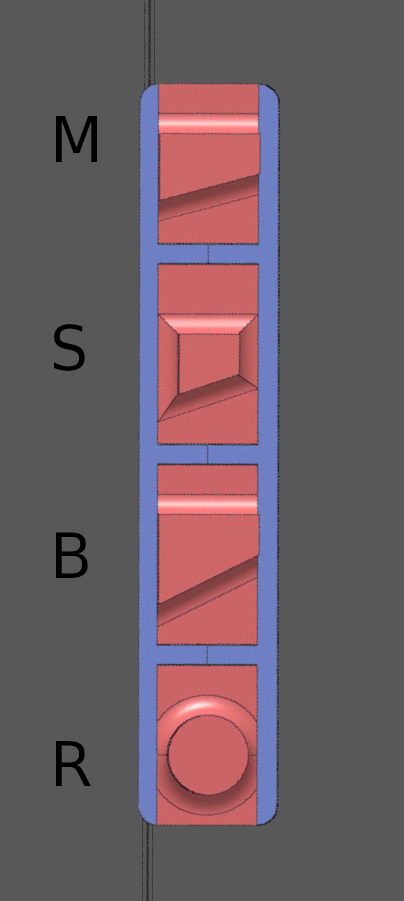
\includegraphics[width=2.1cm]{MAST-U/dsfProbesPlanCroppedLabelled.png}};	
			\node [right=of zoomin] (zoomout){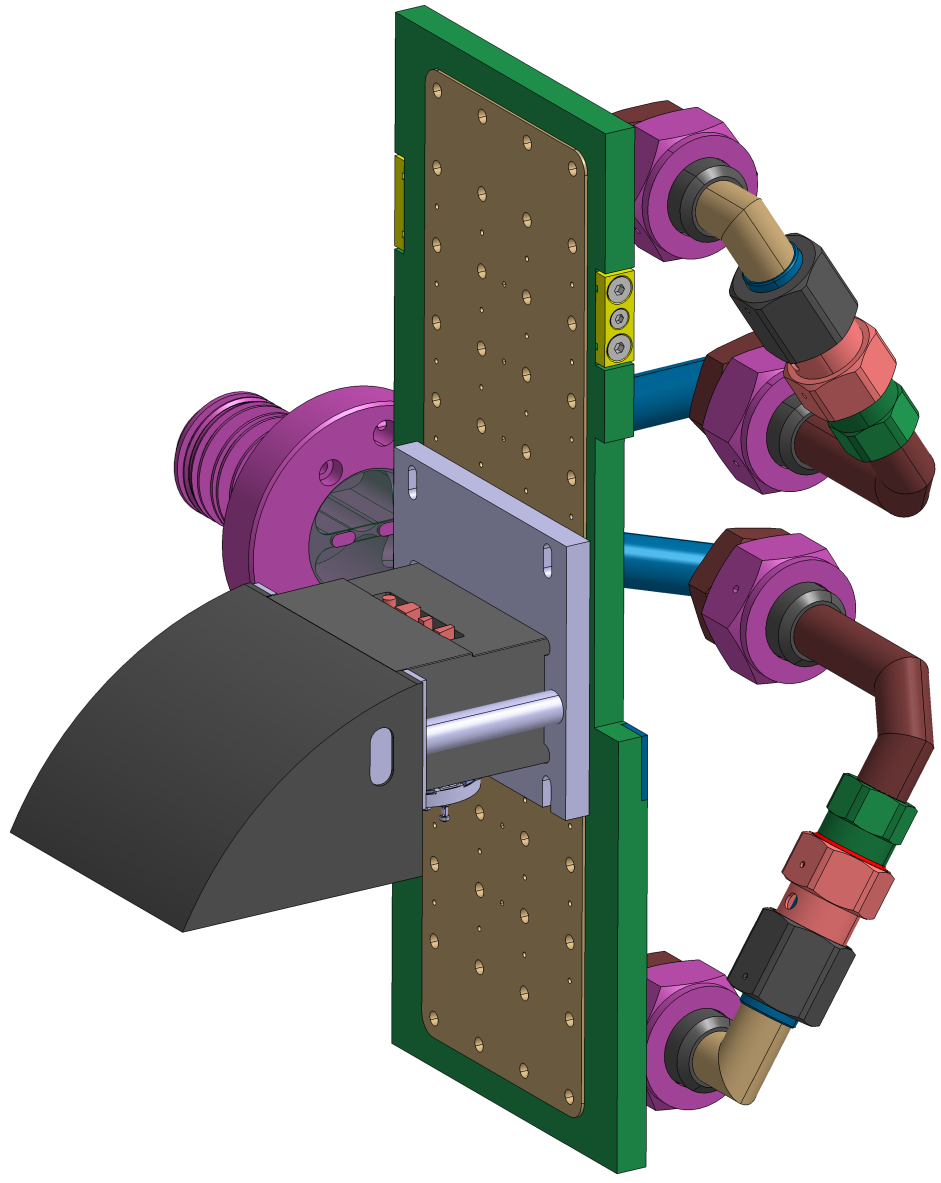
\includegraphics[width=0.4\linewidth]{Magnum/ProbeMountFlip.png}};
%			\draw (2.25,-2.15) to (5.0,-0.35);
%			\draw (2.25,2.15) to (5.0,0.15);
%			\draw (5.0,0.15) rectangle (5.5,-0.35);
			\draw (1.05,-2.34) to (4.2,-0.26);
			\draw (1.05,2.34) to (3.78,0.0);
%			\draw (4.98,-0.0) -- (5.4,-0.26) -- (5.65,-0.21) -- (5.23,0.05) -- cycle;
			\draw (3.78,-0.0) -- (4.2,-0.26) -- (4.45,-0.21) -- (4.03,0.05) -- cycle;
		\end{tikzpicture}
		\caption{\label{fig:dsfprobe}\textit{(left)} CAD schematic of experimental DSF probe head, with four probe tips of differing area and shape. \textit{(right)} CAD schematic of designed mounting system for installing the DSF probe head into Magnum-PSI.}
		\vspace{-10pt}
	\end{wrapfigure}
	Measurements were taken on the linear device Magnum-PSI at DIFFER in Eindhoven, NL, using a 4-probe array designed for the Divertor Science Facility (DSF) at MAST-U with a range of control parameters including incidence angle of magnetic field. 
	A secondary goal of this experiment was to test that these probes performed as expected with regards to minimising sheath expansion and producing expected IV characteristics.
	The remainder of this section describes the experimental setup, analysis techniques used and subsequent results, ending with a discussion on the consequences of this for the interpretation of Langmuir probe data in MAST-U.
%	\begin{figure}[t] % Example image

\subsection{Experimental Method}
	The probe head used in this experiment was a 4-probe array designed for use in the DSF at MAST-U: a sample testing facility installed within the MAST-U divertor which facilitates the exchange of samples or electrical probes while maintaining vessel vacuum \cite{Elmore2012}.
	 
	This probe head has 4 Langmuir probes with tips of different geometry: a standard MAST-U tip, a tip with twice the geometric area of a MAST-U tip, a tip with half the area of a MAST-U tip, and a flush cylindrical probe with similar area to the standard probe. 
	(For reference these will be labelled L, B, S, and R respectively, taken from their designation in the Magnum beam-hall). 
	The first 3 probes are right-trapezoidal in geometry (\cref{fig:dsfprobe}) with the surface of the trapezium angled 10$^{\circ}$ relative to the divertor tile it is recessed into.

	The four probes are electrically isolated from each other by a ceramic pin holder - changed following the previous experiments findings that PEEK was not a suitable material - and the leading edges of the probes shadowed from plasma exposure by a graphite shell around the whole assembly. 
	The distances between the probes and the graphite shell were chosen such that the probe's leading edges are shadowed at incidence angles up to 10$^{\circ}$, the average expected operating regime of MAST-U in Super-X configuration \cite{Harrison}.	
	The same specialised mounting assembly which was designed and manufactured for the previous experiment was used again to hold the DSF probe head in place against the Magnum flat target holder (see \cref{fig:dsfprobe}).
	This target holder is water cooled and could tilt to give a range of magnetic incidence angles onto the probes.
%	The voltage sweep on the probes was produced by an Agilent 3312A arbitrary function generator, the waveform used was a 20Hz triangle wave varying between -100 and +10 V. 
%	This was amplified by a KEPCO 100-4M 100V bipolar operational power supply and applied to two of the four probes at a time. 
%	The current from the probes was measured by using a dual-channel isolational amplifier to observe the voltage drop across two 1$\Omega$ resistors. 
%	All of these signals were then digitised by a National Instruments NI PXI-5105 digitiser, with the voltage signal attenuated 10x to be sampled by the digitiser's 10V range.
%	The digitiser sampled at a minimum rate of 100kHz.
	
	The probes were prepared by vacuum bake at 200$^{\circ}$C for 5 hours, to minimise outgassing. 
	They were exposed to hydrogen plasmas with a range of temperatures and densities, attempting to replicate the conditions within the MAST-U divertor.
	Due to the limitations of the source \cite{DeTemmerman2015a}, the temperatures could not be pushed higher than 3eV while maintaining low enough heat fluxes to prevent secondary electron emission from the LPs\cite{Stangeby2000}. 
	Densities were possible in a range from 2 $\times 10^{19}$ to 2.5 $\times 10^{20}$ m$^{-3}$.
	The angle was varied in all cases between 0 and 10$^{\circ}$, which is the range of angles which are predicted to create challenges for probe interpretation in MAST-U.
	A neutral density scan was performed by increasing pressure in the target chamber using two controls: target chamber pump speed and neutral hydrogen gas puffing at the target location.	
	The plasma and target were also diagnosed with standard Magnum diagnostics: Thomson scattering (TS), infrared imaging (IR) and optical emission spectroscopy (OES). 
	
	\begin{wrapfigure}[23]{lt}{8.5cm}
		\center{
			\vspace{-25pt}
			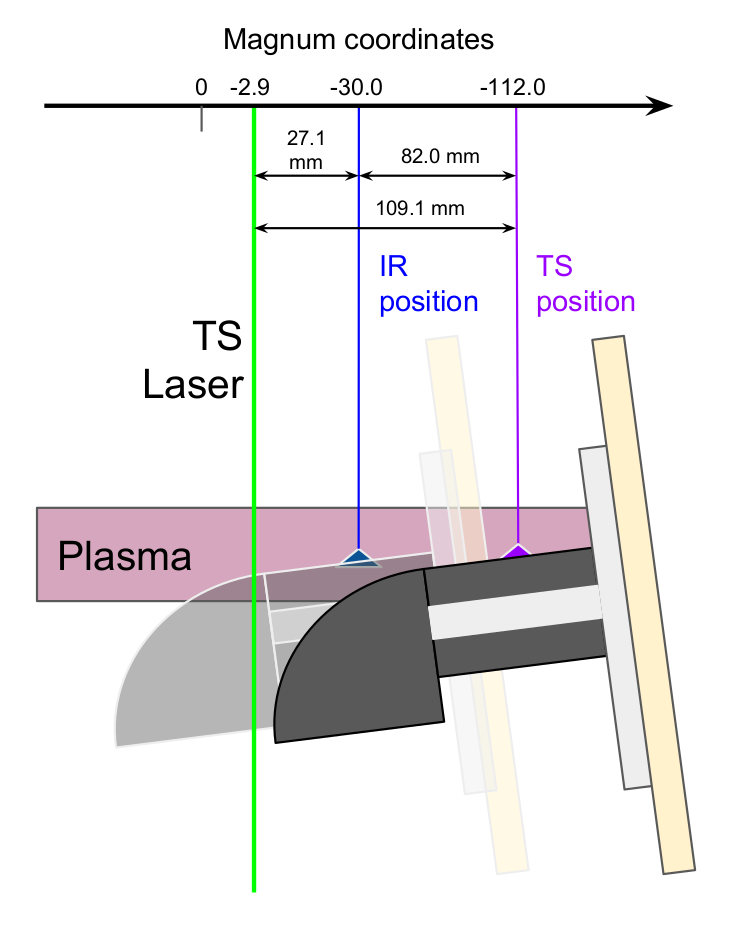
\includegraphics[width=0.90\linewidth]{PRYear2/probeMountGeometry2.png}	
			%			\hspace{15pt}
		}
		\vspace{-5pt}
		\caption{\label{fig:schematic}Schematic diagram showing the location of the DSF probes and mounting system in the Magnum-PSI beam, as well as the relative difference between the IR and TS probe measurement positions, with distances in mm.}
		\vspace{-15pt}
	\end{wrapfigure}
	The TS measured plasma 30mm closer to the source than the probes, and the IR camera was focussed 20mm in the same direction: these measurements were therefore mutually exclusive (see \cref{fig:schematic}) so each set of plasma parameters had to be measured twice at two different axial positions.
	The probes were pushed into position by Magnum's TEAC delivery system for 5-15 seconds at a time with 5 seconds of traversal time either side of this stationary window. 
	
\subsection{DSF Redesign}
%
%	\begin{figure}[b!]
%		\center{
%			\vspace{-15pt}
%			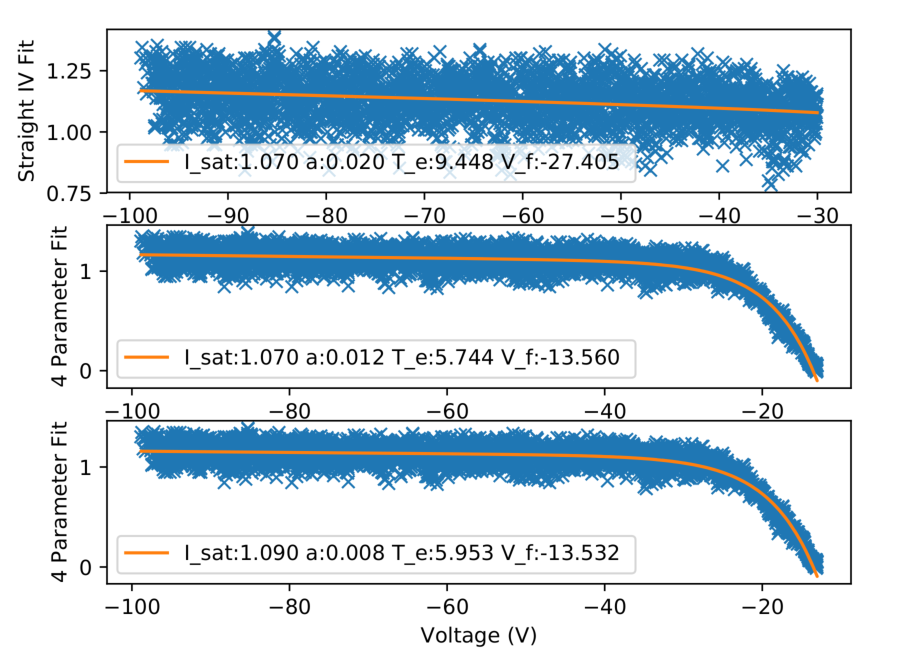
\includegraphics[width=1.0\linewidth]{CollabReport/threeStageFit_cropped.pdf}
%		}
%		\vspace{-15pt}
%		\caption{The 3 stages of fitting used in analysis of IV characteristics: the straight saturation region fit (top), the fixed $I_{sat}$ fit (middle) and the full, freely varying fit (bottom).}
%		\label{fig:threeStageFit}
%		\vspace{-15pt}
%	\end{figure}
	A key finding from the experiment was the discovery of two design flaws with the DSF probe-head stemming from the choice of PEEK as the pin-holder material.
	Firstly, upon vacuum-baking it was evident that there was insufficient space between the graphite shell and the PEEK pin-holder to account for the difference in thermal expansion coefficient of the two materials.
	This led to the cracking of the graphite shell into 3 pieces.
	The design for the DSF has been updated, with the PEEK pin-holder being replaced with ceramic to prevent this from occurring.
	Secondly, the surface temperatures of the probes and graphite shell were high enough to cause the PEEK to melt.
	Molten PEEK then seeped into the gaps between the probes and the graphite shell, becoming exposed to plasma and burning. 
	This PEEK ash was then sufficiently electrically conductive that it created a short between two of the probes and the graphite shell, prohibiting their use until they could be taken out of the machine and the conductive material removed.
	The surface temperature of the assembly was much higher than it will be in MAST-U due to both the longer exposure times of the Magnum setup and the unfortunate existence of an exposed leading edge on the interface between the mounting device and the DSF probe head. 
	The latter was confirmed by the appearance of a hotspot on the IR camera of up to 1600$^{\circ}$C depending on incidence angle.
	Both of these will not be present when operating in MAST-U however, as the heat fluxes will be much lower, but the change to a ceramic pin-holder has also fixed this problem for future experiments on Magnum-PSI. 
	The leading edge on the probe mount will require modifications to the Tungsten back-plate to remedy in future experiments.

\subsection{Results}
	\begin{figure}[b!]
		\center{
			\vspace{-20pt}
			\subfloat[]{\label{fig:threeStageFit}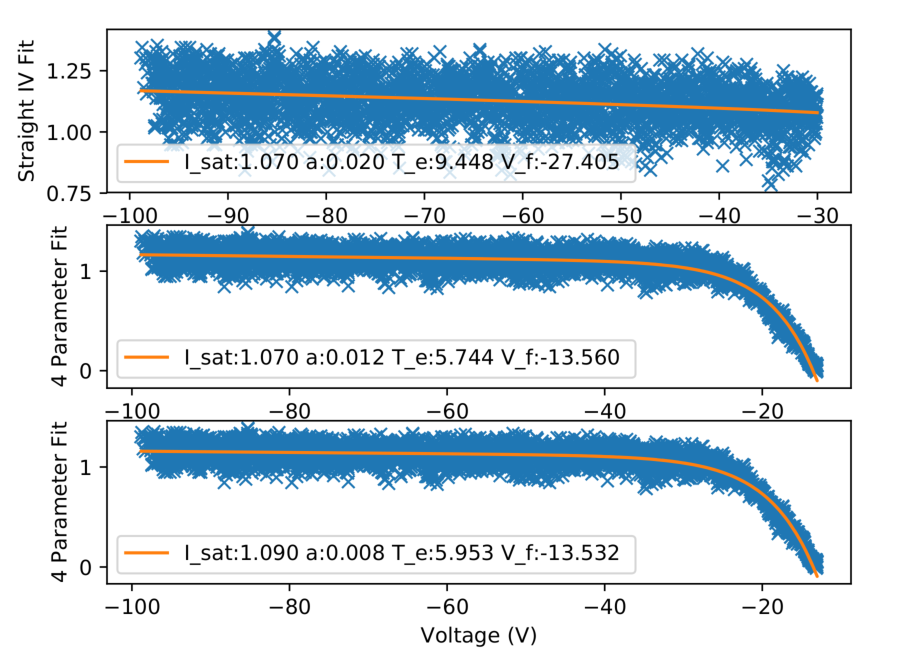
\includegraphics[width=0.485\linewidth]{CollabReport/threeStageFit_cropped.pdf}}
			%			\hspace{2pt}
			\subfloat[]{\vspace{-1pt}\label{fig:ivComparison}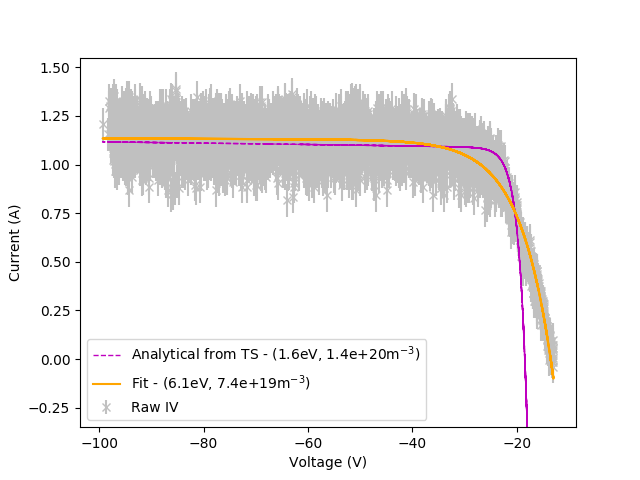
\includegraphics[width=0.513\linewidth]{PRYear2/ivComparison2.png}}
		}
		\vspace{-0pt}
		\caption{
			(a) The 3 stages of fitting used in analysis of IV characteristics: the straight saturation region fit (top), the fixed $I_{sat}$ fit (middle) and the full, freely varying fit (bottom).
			(b) Comparison of fitted IV curve to IV curves generated using the 	analytical formula from measured TS values. 
			The 'Analytical from TS' shows a much sharper knee associated with lower $T_e$, but approximately equivalent $I_{sat}$. 
			%			Most interestingly, the 'Analytical - measured' curve in red shows that the sheath expansion parameter calculated using coefficients $c_1$ and $c_2$ from \cite{Murphy-Sugrue2017a} slightly underestimates the amount of sheath expansion observed from the DSF probe measurements. 
			%			This can be seen in the difference in gradient in the ion saturation region of the IV curve.
		}
		\vspace{-15pt}
	\end{figure}
	Due to a fault with the Langmuir probe electronics, the most reliable data was obtained during the scan of neutral gas puffing - as such these results will be discussed in detail.
	These measurements were taken at an incidence angle of 10$^{\circ}$.
	The half area probe (S) is used in all measurements discussed as it was approximately in the centre of the plasma beam and did not short during the experiment.
	A low-pass Butterworth filter with a critical frequency of 4kHz was applied to the voltage signal to remove high frequency noise.
	
	IV characteristics were analysed using the 3-stage method developed on MAST \cref{fig:threeStageFit}.
	The full 4-parameter model was used throughout (\cref{eq:ivcurvesheathexp}), parameters being $T_e$, $I_{sat}$, $V_f$ and $a$.
	The ion saturation region of the IV curve is fit first to get an initial value for ion saturation current.
	This initial value of $I_{sat}$ is then kept fixed in a second, 4-parameter fit to the whole IV curve. 
	Finally, a full, freely varying 4-parameter fit is carried out, with initial values taken from the second fit, to get final parameter values and uncertainties.
	Comparisons were made between a 3- and 4-parameter fit and only small differences in the fitted value of $I_{sat}$ were found, which provides good evidence that the DSF probe tip's tilted design is successfully reducing sheath expansion effects at larger angles.
	Densities were calculated from the fitted parameters using the definition of ion saturation current $I_{sat} = n_e e c_s A_{eff}$, 
	%	\begin{equation}
	%	% Modified I_sat definition
	%	\label{eq:isateffective}
	%	I_{sat} = n_e e c_s A_{eff}
	%	\end{equation}
	where $c_s$ is the sound speed and $A_{eff}$ is the effective collection area of the probe - in this case taken as the projected area along the field line, found by extending the derivation of the exposed probe extent (in \cite{Harrison}) to right trapezoidal geometry.
	$c_s$ is calculated from $c_s = \sqrt{\frac{e(T_e + T_i)}{m_i}}$ and $T_e = T_i$ assumed. 
%	The form of $A_{eff}$ for probes S, M, and B, is then given by:
%	\begin{equation}
%	% IV Curve
%	\label{eq:a_eff_alternate}
%	A_{eff} = \frac{1}{2} \bigg(a + b - \frac{d}{\tan{\theta_{f}}} \bigg)\bigg(\frac{L}{\cos{\theta_{p}}} - d\bigg) \sin{\Big[|\theta_{\perp}| + |\theta_{p}|\Big]} + b \cos{\theta_{p}}\Big(d_{\phi}\tan{\theta_{\perp}} - d_{\perp}\Big)
%	\end{equation}
%	\begin{equation}
%	% IV Curve
%	\label{eq:d}
%	d = \frac{d_{\perp} - d_{\phi}\tan{\theta_{\perp}}}{ \sin{\theta_{p}} + \tan{\theta_{\perp}}\cos{\theta_{p}}}
%	\end{equation}
	\begin{figure}[t!]
		\center{
			\vspace{-20pt}
			\subfloat[]{\label{fig:densityScan_Tn}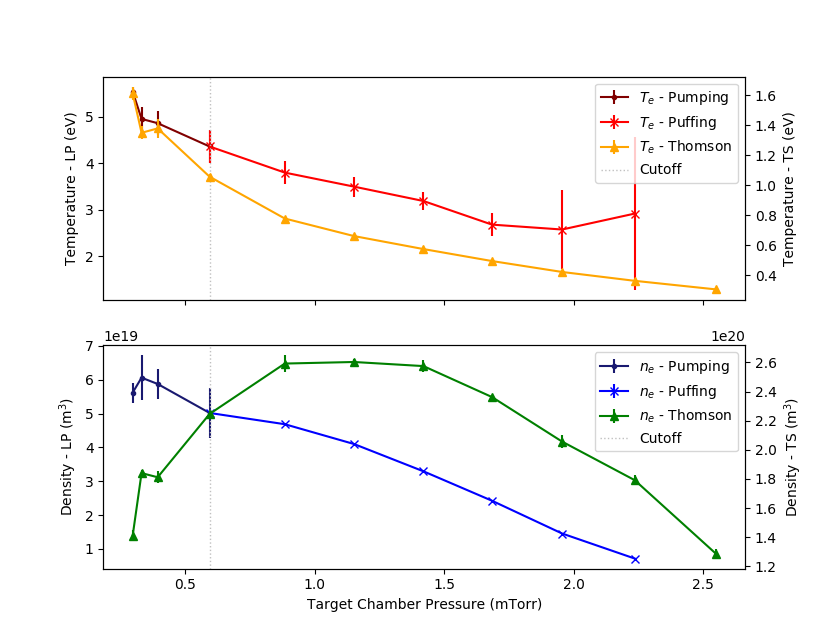
\includegraphics[width=0.49\linewidth]{CollabReport/densityScan_TeNe_TS.png}}
			\subfloat[]{\label{fig:densityScan_jq}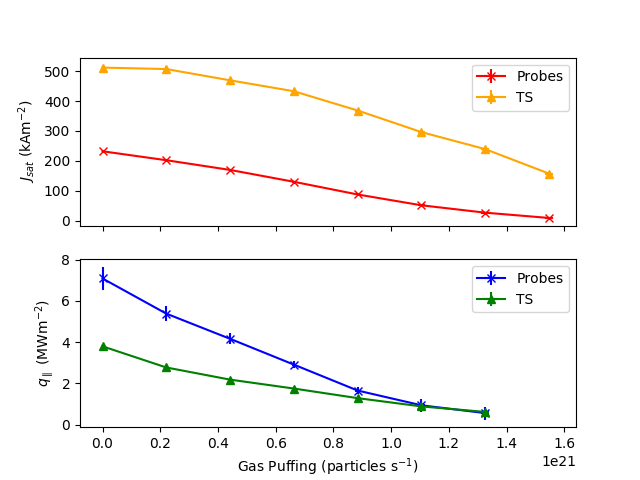
\includegraphics[width=0.51\linewidth]{CollabReport/densityScan_jsatQpar_TS.png}}
		}
		\vspace{-5pt}
		\caption{
			(a) Graph of measured $T_e$ and $n_e$ from DSF 'S' probe and TS system as a function of target chamber pressure. 
			The 'cutoff' listed above is the point at which pump speed reduction was stopped and gas puffing began. 
			%			Note the peak in the TS density profile, which may indicate the existence of a detachment front moving along the beam from the probes to the TS system.
			(b) Graph of $J_{sat}$ \textit{(upper)} and $q_{\parallel}$ \textit{(lower)} calculated from probe measurements and TS data as a function of gas puffing speed.
		}
		\vspace{-15pt}
	\end{figure}
	
	When comparing results from the LPs with $T_e$ and $n_e$ measured by the TS system, a systematic overestimation of temperature was found by the LPs along with systematic underestimation of density.
	Analytical IV characteristics were created from the TS data (\cref{fig:ivComparison}) approximating $V_f \sim 3 T_e$\cite{Stangeby2000} and calculating $a$ from \cref{eq:sheathexpparam}, substituting in Murphy-Sugrues values for the constants $c_1$ and $c_2$ (although this made little difference to the overall shape of the IV as $a$ was very small in most cases).
	
	The density difference could be explained by a decreasing density profile along the magnetic axis of the beam between the TS laser and the probes, which is unfortunately difficult to verify as there is little available data about the axial profiles of density and temperature on Magnum-PSI due to the static nature of the available diagnostics.
	Preliminary analysis of the probe measurements taken in the 5 second traversal time either side of the stationary measurement window found there to be an increase of density as the probes moved into position, but further analysis would be required to draw conclusions about the exact nature of this profile.
	The temperature difference does not have a clear explanation, as great care was taken to ensure the 4-parameter fit was as good as possible - achieved by ensuring errors were not overestimated through reduced $\chi^2$ goodness-of-fit testing and optimising the range of fitted data in voltage-current space.
%	Potential explanations of this finding could be found by challenging underlying assumptions: notably the electron-ion temperature equivalence which is at the core of Langmuir probe theory.
	The best current explanation is that the TS beam was not aligned properly down the centre of the plasma beam and was therefore providing an off-axis temperature reading, i.e. not measuring through the hottest section of the beam.
	Langmuir probes are however documented as being difficult to use on plasmas at temperatures on the order of a few eV\cite{Stangeby2000}, especially in noisy environments like tokamaks and linear devices, and this could be an explanation for the disparity of the temperature measurement.
%	Magnum-PSI is in the process of implementing a collective Thomson scattering (CTS) system which could, when working, provide a measurement of $T_i$ and validate the former point. 
%	The latter point is more difficult to validate, and would require greater plasma diagnosis closer to the FMPs (e.g. closer TS measurements).
%	It could also be the case that the temperature measurement is in fact correct due to some as-yet unknown plasma physics happening between the probes and the TS laser.
	
	Analysis of the density scan was conducted using the measured temperatures and densities and comparing their profiles to those measured by the TS system. 
	Saturation current density ($J_{sat}$) and parallel heat flux ($q_{\parallel}$) were also measured, with the latter using a value for the sheath heat transfer coefficient ($\gamma$) as 7.
%	Results show a continually decreasing temperature and density profile seen by the probes, as expected, but a roll-over in the TS density profile (\cref{fig:densityScan_Tn}). 
%	This rollover, along with the difference in position of the diagnostics, may indicate the movement of a detachment front up the beam as gas puffing is increased.
%	An explanation could be that as more gas is pumped into the chamber the plasma closer to the probes is more readily detached, causing the initial plasma density drop off seen by the probes. 
%	%	potentially because of the increased neutral density in front of the probe surface,
%	The plasma at the TS position requires more neutral density to see the drop off in plasma density take effect, resulting in the rollover of density at a higher value of target chamber neutral pressure.
%	\begin{figure}[!tb]
%		\center{
%			\vspace{-20pt}
%			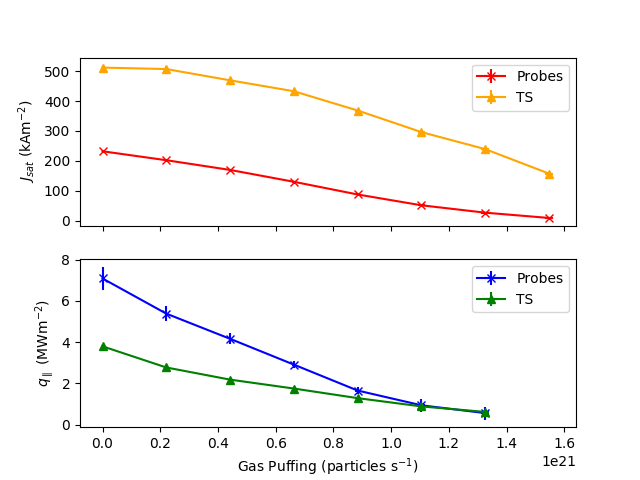
\includegraphics[width=.8\linewidth]{CollabReport/densityScan_jsatQpar_TS.png}
%		}
%		\vspace{-0pt}
%		\caption{
%			Graph of $J_{sat}$ \textit{(upper)} and $q_{\parallel}$ \textit{(lower)} calculated from probe measurements and TS data as a function of gas puffing speed. 
%%			Delayed onset in reduction of $J_{sat}$ supports previous measurements in suggesting the existence of a moving detachment front.
%			%			Good agreement between the reduced heat flux at higher gas puff rates, suggests a saturation of the heat mitigation effect of higher neutral density.
%		}
%		\label{fig:densityScan_jq}
%		\vspace{-15pt}
%	\end{figure}
	The $J_{sat}$ and $q_{\parallel}$ profiles \cref{fig:densityScan_jq} show a continuous decline as neutral density increases, as would be expected due to the plasma-neutral collisions reducing the energy of plasma particles before they reach the probes.
	This could be considered an indicator of detachment and, if so, would be accompanied by an increase in radiation from the plasma in front of the probes. 
	This could be verified in further experiments.
	The delayed onset in the reduction of $J_{sat}$ in the TS measurements (i.e. further along the beam) may suggest the area of increased collisions is moving up the beam.
	Agreement can be seen between the probe and TS measurements of $q_{\parallel}$ at higher levels of gas puffing, however this is likely due to the overestimation of $T_e$ and underestimation of $n_e$ combining fortuitously.
%	This agreement also suggests that the high temperatures measured by the probes are physical and reduced to the normal levels by the decrease in heat flux due to neutral gas puffing.
	%	The values of heat flux are slightly higher than expected, as one would expect to find o, suggesting that the overestimation of temperatures is not a physical phenomenon but an issue with the interpretation of the IV curves.
	
	IR camera data is still pending thorough analysis, but could be used to verify the heat flux measurements.

%------------------------------------------------------------------------------------
%	PhD Project Plan
%------------------------------------------------------------------------------------

\section{\label{sec:phd}Future Work \& Plan}

%\subsection{\label{subsec:simulations}Return to Magnum-PSI}
	The work carried out on Magnum-PSI, while fruitful, is incomplete.
	A further experiment has therefore been requested to complete the following goals: (a) carry out the investigation of incidence angle dependence on probe measurements, and (b) test the new design of the DSF probe head to ensure the previously uncovered problems have been remedied.
	For this investigation a week of beam time has been requested and the experiment will be carried out in collaboration with another PhD student at CCFE hoping to test the efficacy of a new diagnostic: coherence imaging spectroscopy.
	This will provide measurements of temperature and density to have a further diagnostic to compare probe measurements to. 
	It has also been requested that the electronics used in the previous experiment be re-used to minimise the introduction of additional noise or interference effects.

%\subsection{\label{subsec:experiments}JET Simulations}
%It has also been suggested that the justification for the
	Verification, with detailed simulation on SPICE, of the 4-parameter fit used in the fitting of FMP data on the Joint European Torus (JET) at CCFE is also planned for next year.
%	The model is used on all data regardless of magnetic incidence angle and verification as to whether the modified 4-parameter fit \cite{Gunn1995} would be useful for future probe analysis; both for JET and for MAST-U, as the angled probe tip design was based on the probes at JET.  
	This work will take the form of simulating JET probe tips under a variety of JET relevant conditions - most likely from looking at plasma parameters from high quality JET LP shots - and then comparing the simulation results to the IV characteristics in the JET database. 
	This will establish whether it was valid to use the 4-parameter fit in all previous JET data and advise on whether to continue using it, or alternatively the simplified 3-parameter fit, on upcoming campaigns.
%	The shots will be chosen based on how applicable the 4-parameter fit appears to be for that shot, with a range of highly suitable and unsuitable shots chosen.
%	This will hopefully give a good idea of whether the 4-parameter fit is (a) computationally reproducible, and (b) of limited use in certain areas of parameter space.

%\subsection{\label{subsec:}Conferences}

%\subsection{\label{subsec:timeline}Timeline for Remainder of PhD}

	The overall plan for the remaining 2 years of research, i.e. Dec 2018 - Sep 2020, has been drafted in \cref{fig:timeline}.
	\begin{figure}[t]
		\center{
			\vspace{-15pt}
			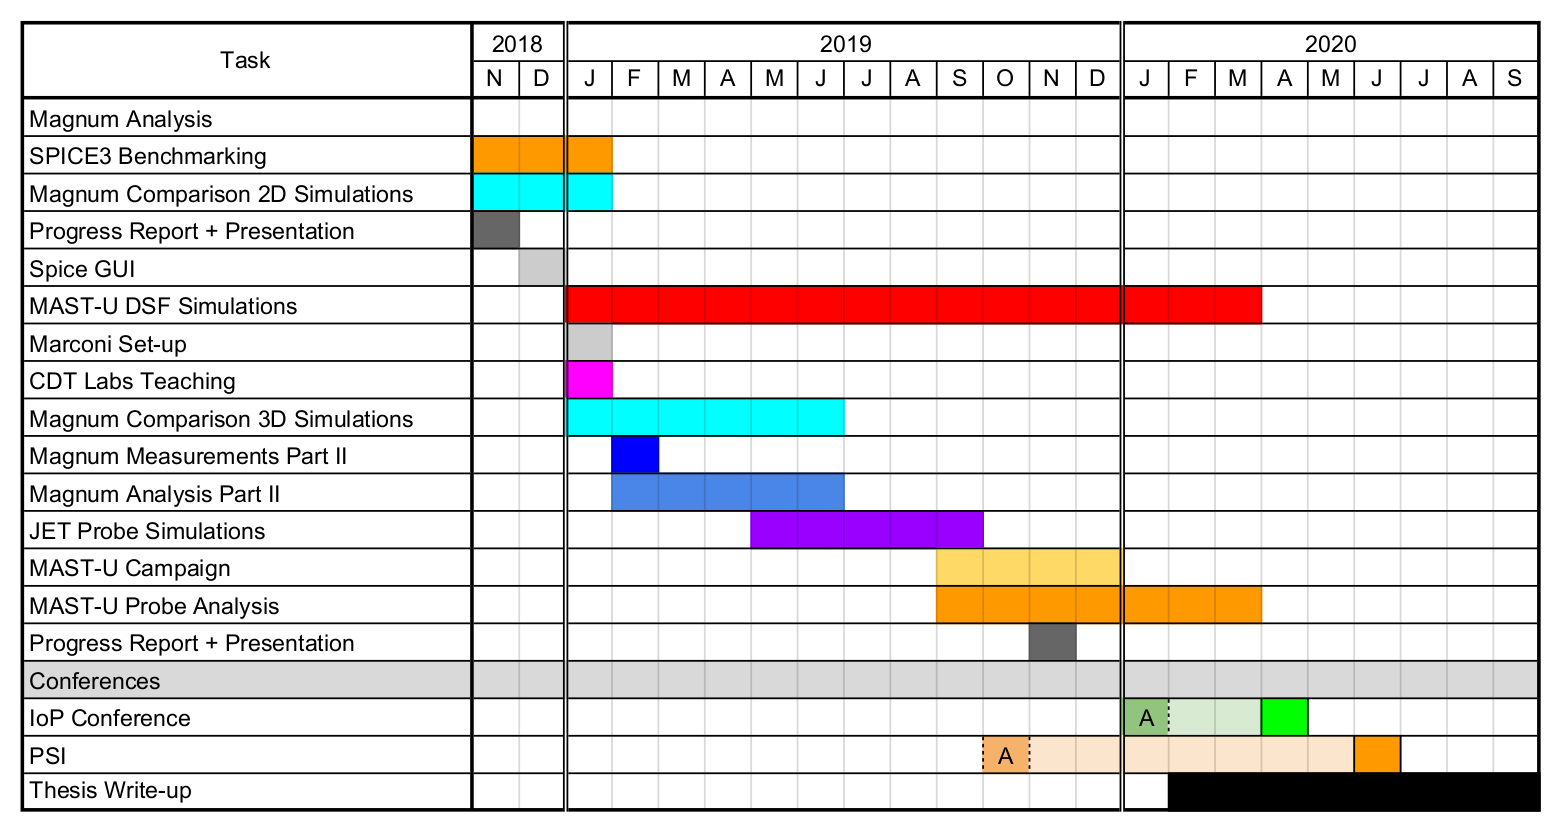
\includegraphics[width=0.8\linewidth]{PRYear2/plan3.png}
		}
		\vspace{-0pt}
		\caption{A Gantt chart denoting breakdown of proposed work and milestones to achieve. Squares marked A denote the submission deadline for the respective conference abstract.}
		\label{fig:timeline} 
	\end{figure}
	This is not finalised but is intended to give an overall impression of the desired work and how long it will take. 
%	Three papers are intended to be published on the three overall areas of the PhD project: MAST-U LPs, JET LPs and Magnum-PSI measurements. 
	Two conferences are currently planned to be attended: plasma surface interactions (PSI) and the IoP plasma physics conference in 2020.
	I plan to present a poster at PSI, and as part of the conference I will utilise the opportunity to submit a paper for publication in the conference proceedings journal.
	Other conferences will be considered, such as the APS and EPS conferences in the US and Europe respectively, depending on available budget.
	A second trip to Prague for assistance in analysing SPICE data from larger simulations, is also planned for some point in the remaining 2 years. 
%	This will use the majority of my remaining conference budget, with further small conferences possibly to be attended if ad-hoc funding can be found. 


%----------------------------------------------------------------------------------------
%	BIBLIOGRAPHY
%----------------------------------------------------------------------------------------

\begingroup
\setstretch{0.8}
\setlength\bibitemsep{3.5pt}
\printbibliography
\endgroup
%
%\bibliography{sample}

%----------------------------------------------------------------------------------------

\end{document}